
\chapter{L2 - All About Processes}
This chapter provides an overview of the fundamental concepts underlying modern process management and memory organization in computer systems. We discuss multithreading, CPU registers, the role of compilers, and memory organization—including both stack and heap memory—as well as virtualization techniques that allow multiple processes to coexist seamlessly.
\small
\section{Multithreading}
When a program runs, the processor loads it into main memory and creates a thread. In a multithreaded program, there is typically one \emph{manager} thread that delegates work to several \emph{worker} threads. For instance, when computing the sum of a large set of numbers, the workload can be divided into subsets, with each worker thread processing a portion of the data while the manager coordinates the overall computation.

\begin{center}
    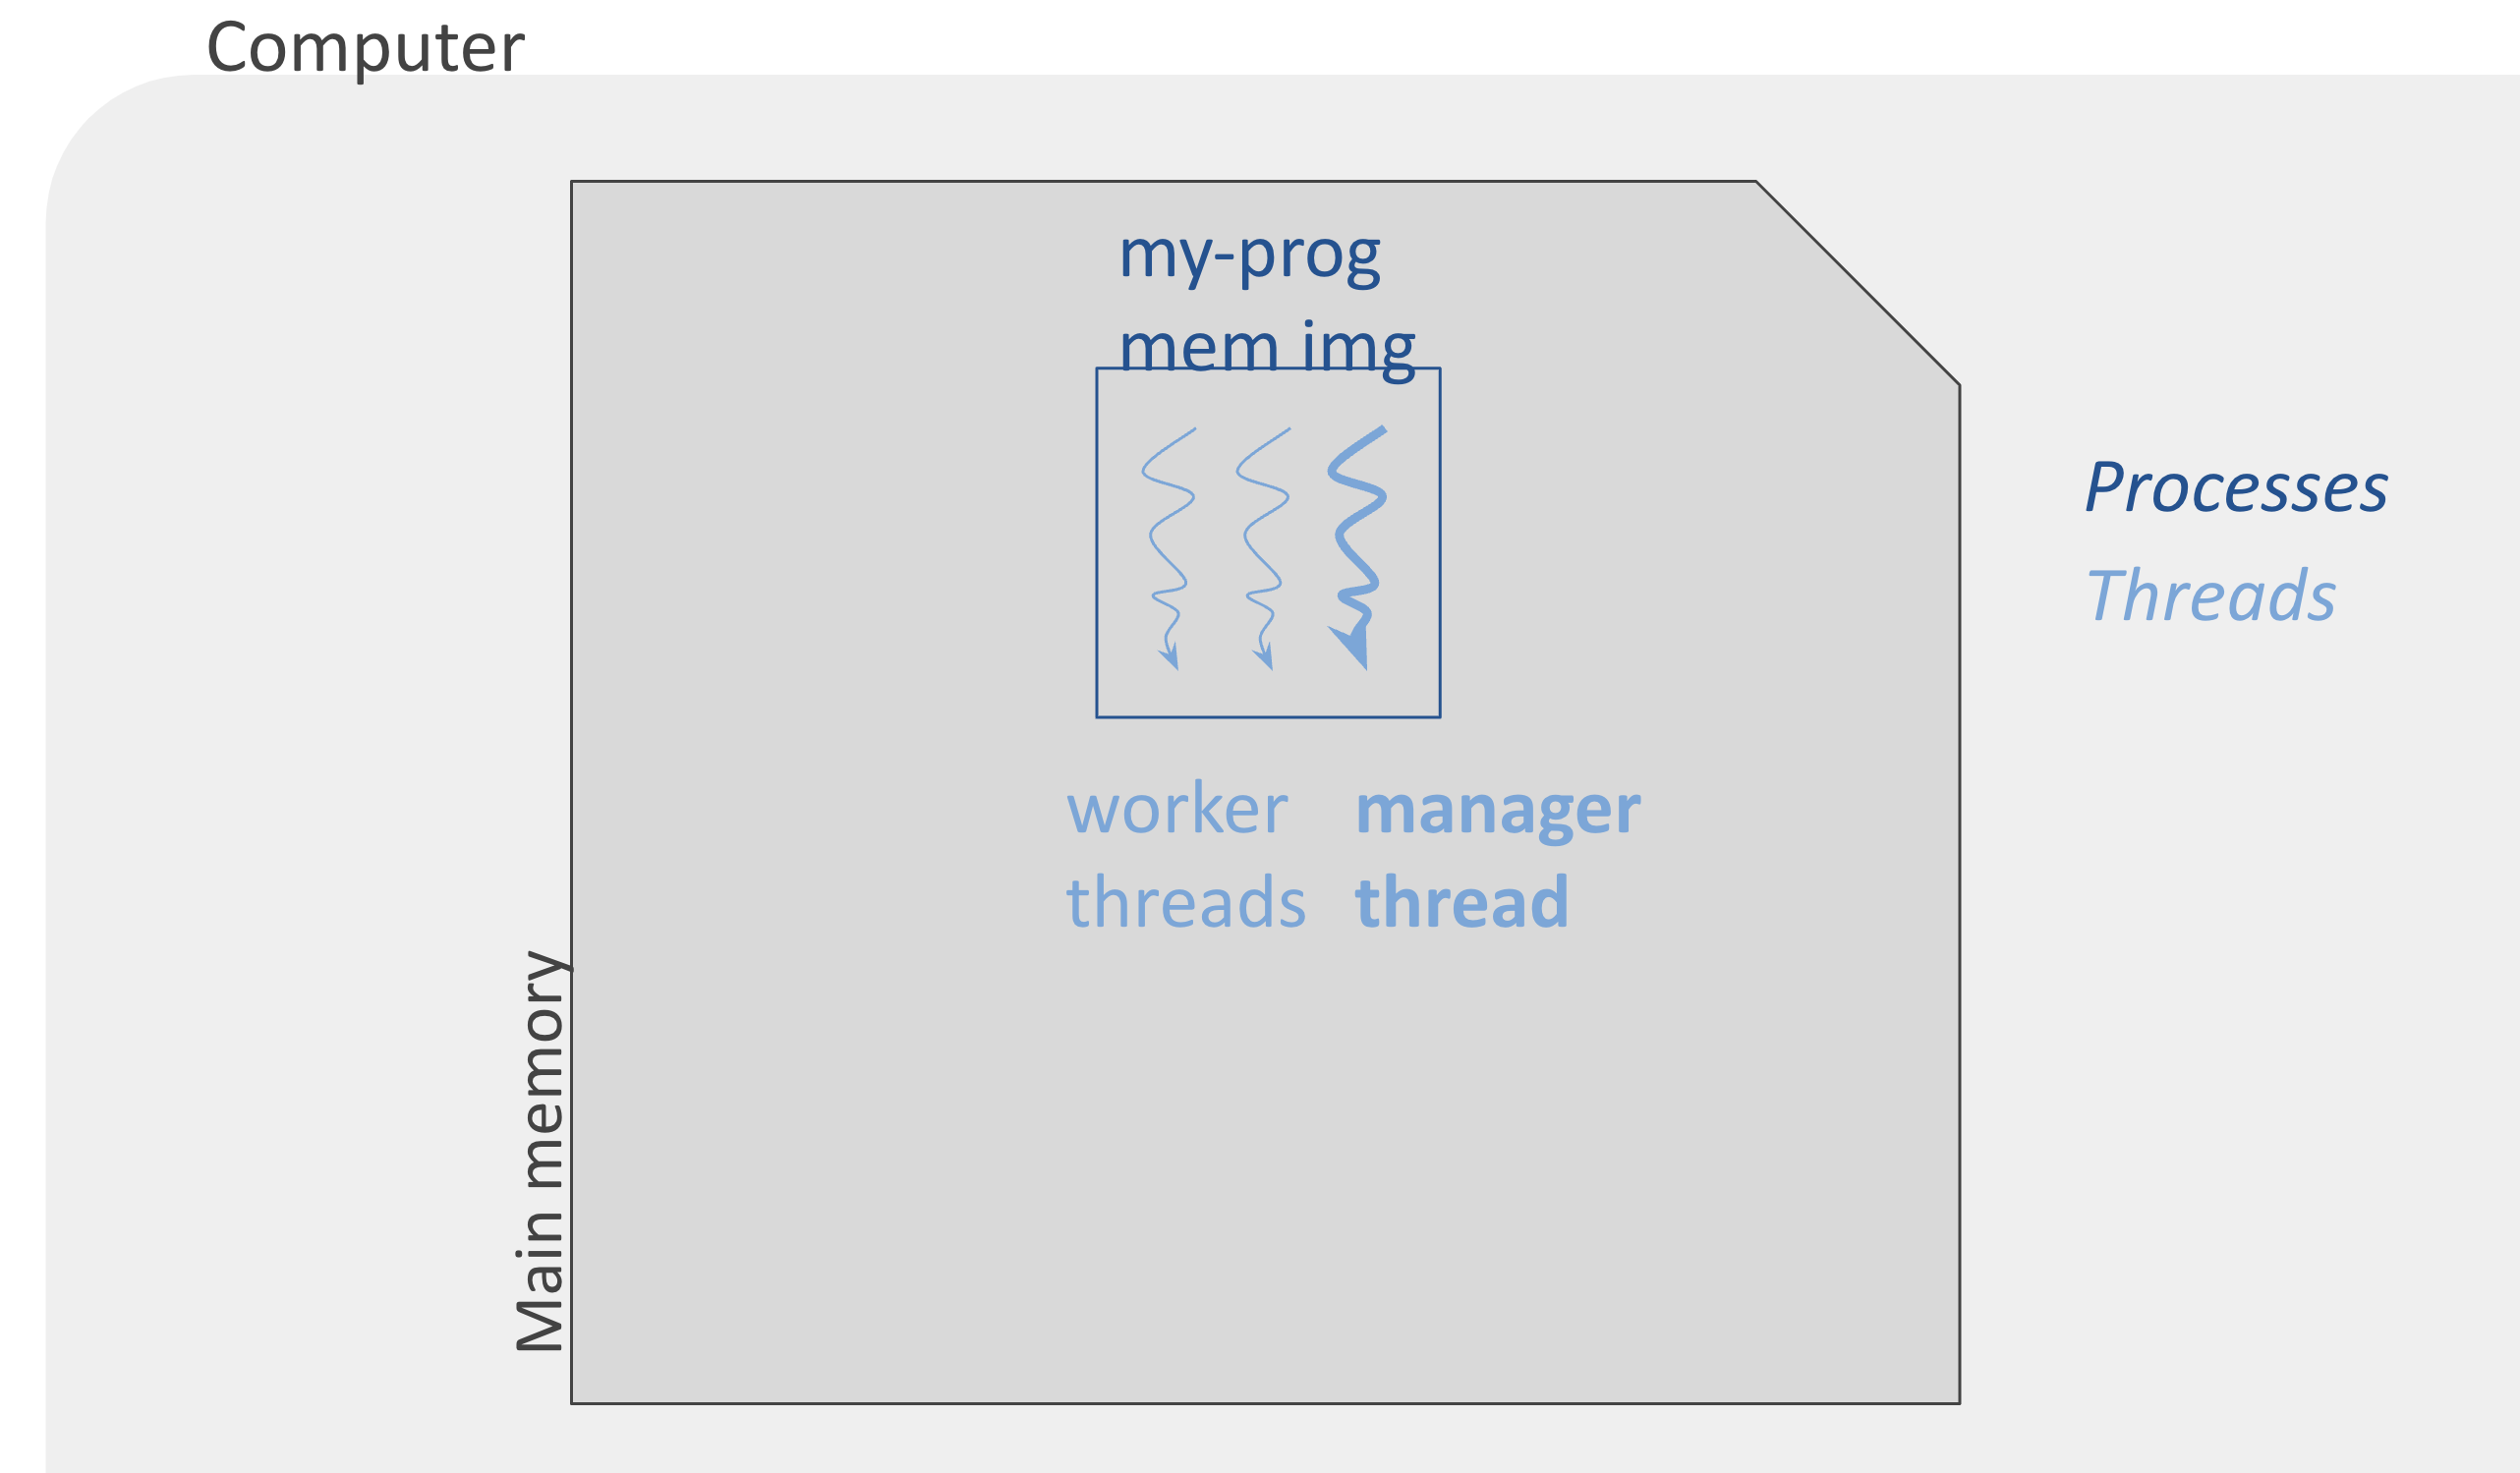
\includegraphics[width=0.55\textwidth]{chapters/L2/images/multi_threads.png}
\end{center}

\section{Registers}
\begin{minipage}{0.45\textwidth}
CPU registers are small storage locations within the processor that hold data and instructions needed during execution. For example, the \texttt{mov} instruction might transfer data from one register (or memory location) to another. Key registers include:
\begin{itemize}
  \item[-] \textbf{Instruction Pointer (IP):} Keeps track of the next instruction to be executed.
  \item[-] \textbf{Stack Pointer (SP):} Points to the current top of the stack in main memory.
\end{itemize}
\end{minipage}
\hfill
\vline
\hfill
\begin{minipage}{0.45\textwidth} 
\begin{center}
    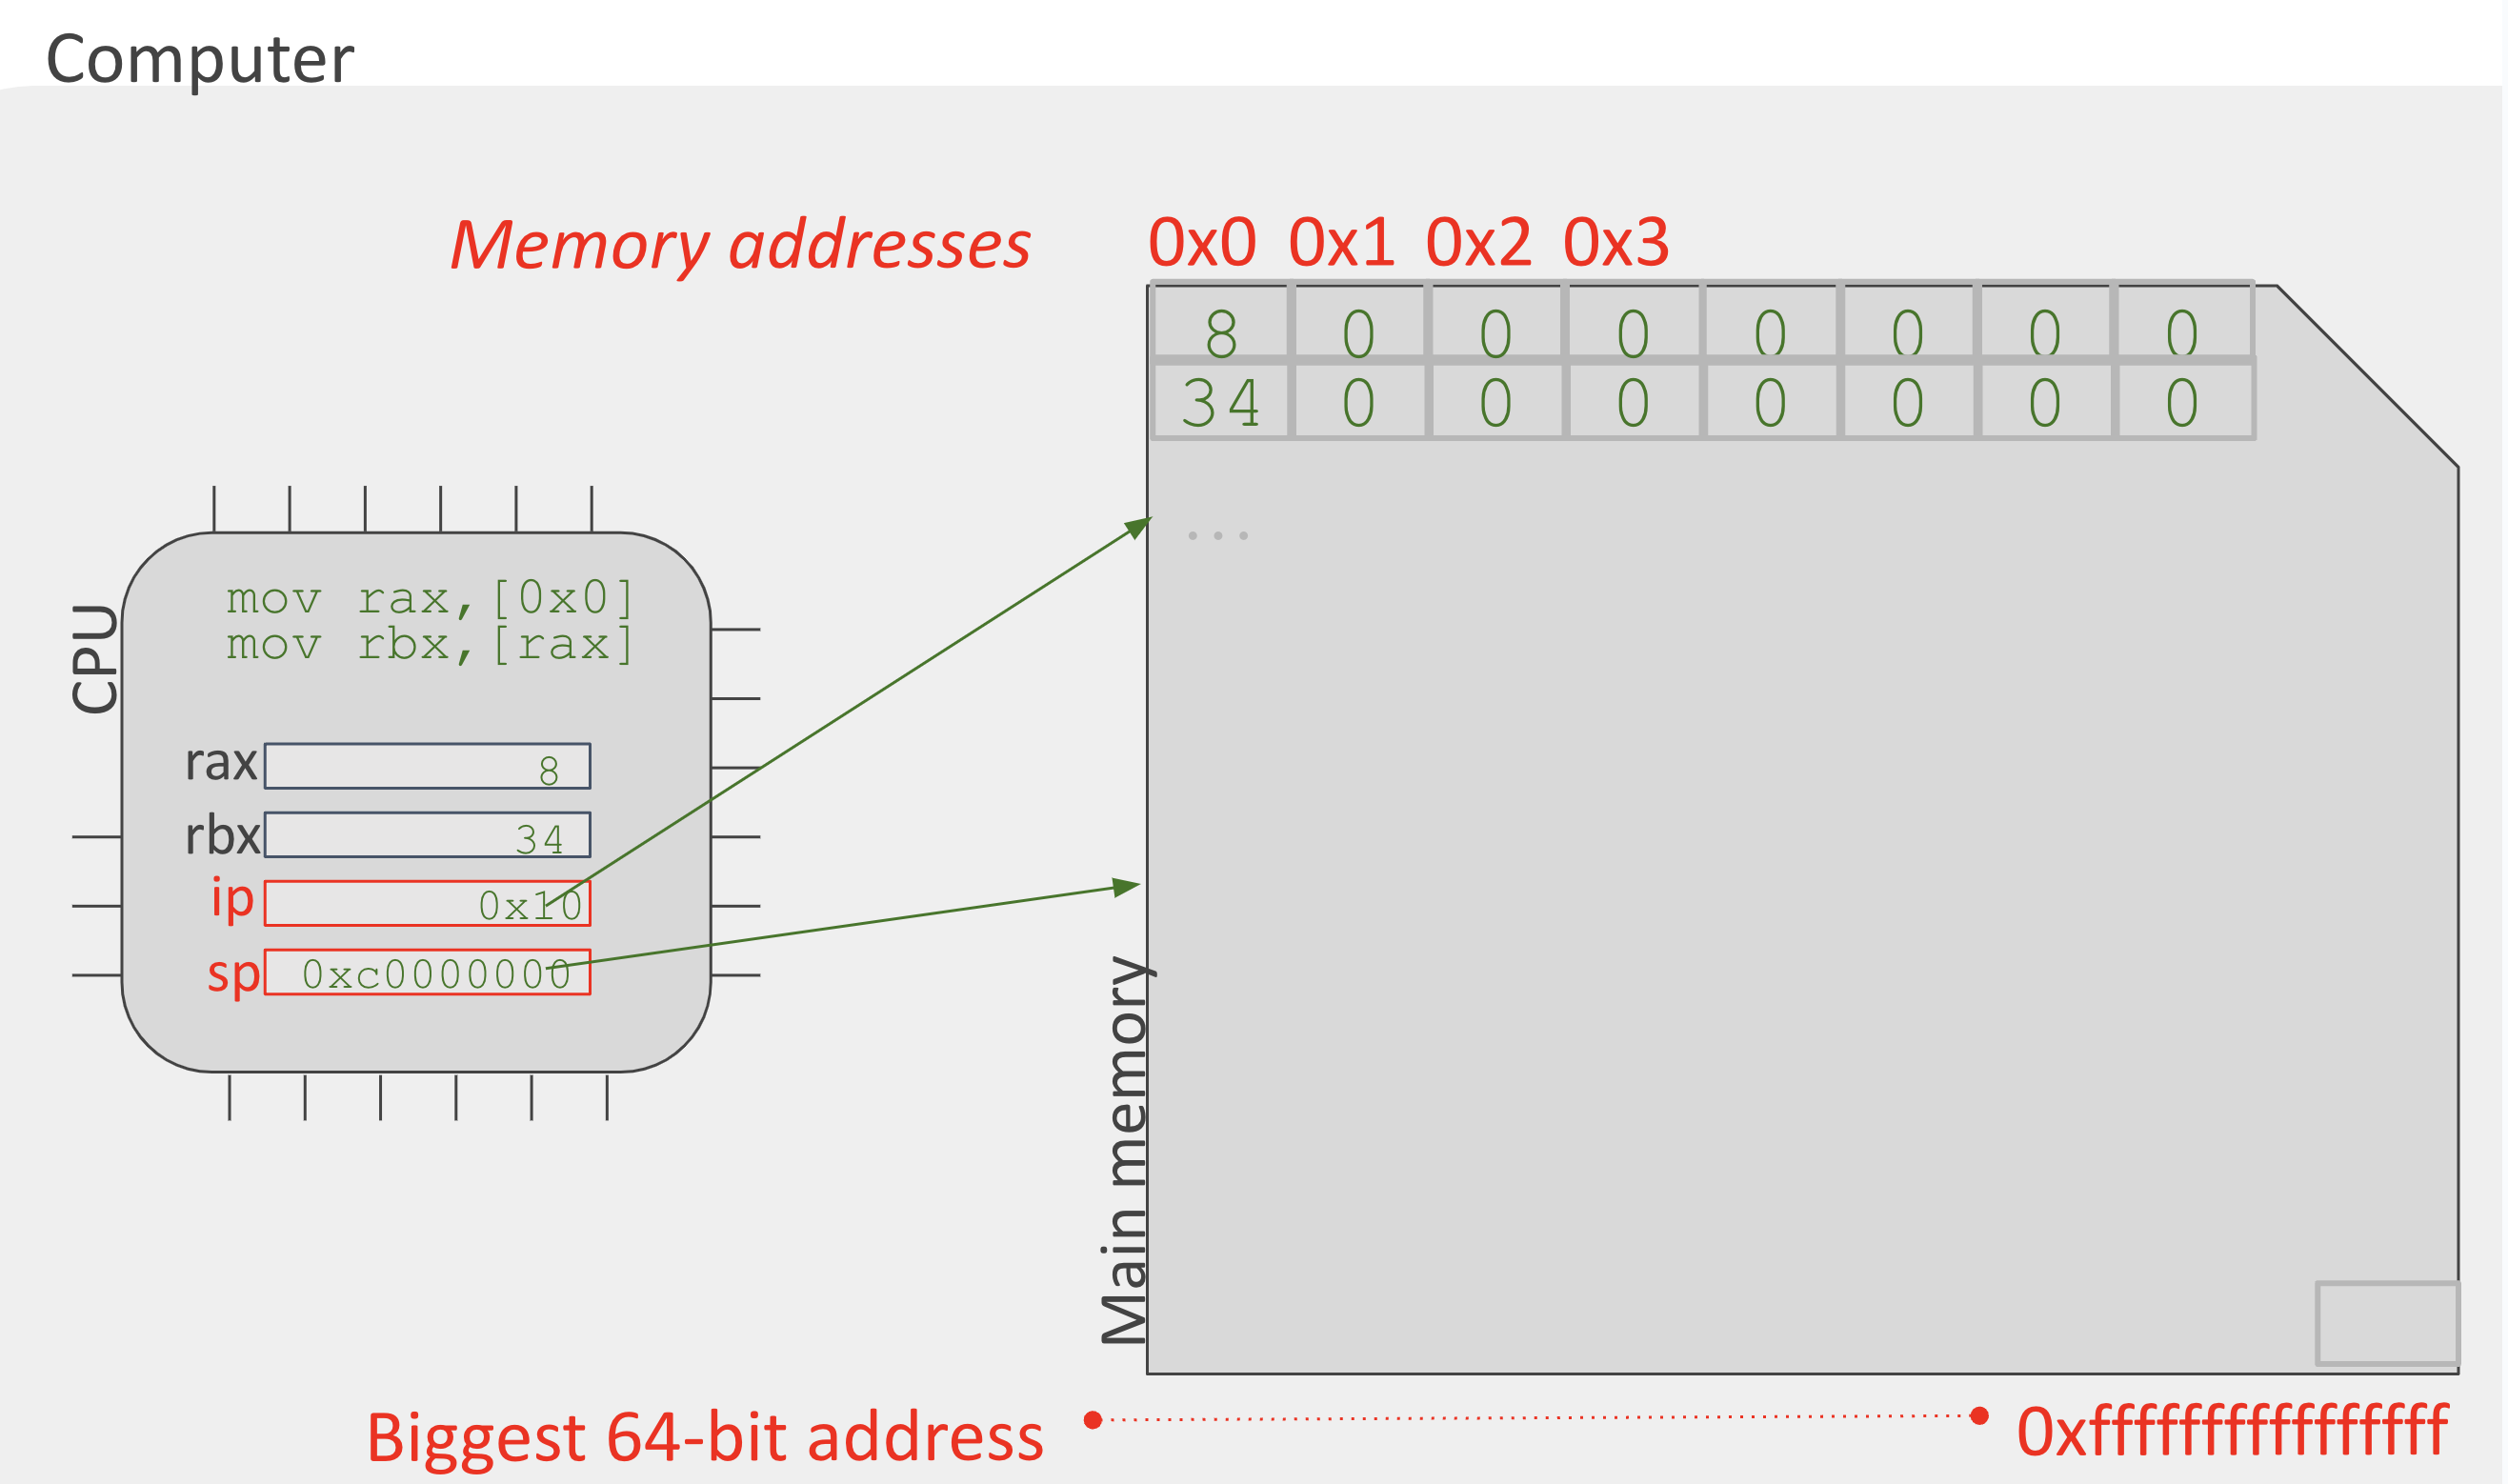
\includegraphics[width=1.1\textwidth]{chapters/L2/images/registers.png}
\end{center}
\end{minipage}
\newpage
\begin{definition}[Compiler]
A compiler translates high-level source code (such as C) into low-level executable code (often Assembly language). This translation involves parsing, optimization, and the generation of machine-specific instructions.
\end{definition}

\section{Memory Organization}
\textit{I'll go a little bit deeper for our fellow syscoms, I also recommend understanding how LIFO works before reading this, if you're too lazy for that, it's basically in the name Last In First Out, means that the last item pushed onto the stack is the first one to be removed, just like stacking plates— you take the top plate first before reaching the ones below. } \\
In modern computer architectures, a process's memory is divided into several distinct segments, each serving a specific role during program execution. Understanding these segments is fundamental for effective programming and debugging. \\[10px]

\begin{definition}[Memory Segments]
A process's memory image is typically divided into the following segments:
\begin{itemize}
    \item \textbf{Text Segment:} Contains the executable code and embedded constants. It is usually marked as read-only to prevent accidental modification.
    \item \textbf{Data Segment:} Stores global and static variables. This segment is often subdivided into:
        \begin{itemize}
            \item \textbf{Initialized Data:} Variables explicitly initialized by the programmer.
            \item \textbf{Uninitialized Data (BSS):} Variables that are declared but not explicitly initialized, and are set to zero by default.
        \end{itemize}
    \item \textbf{Heap Segment:} Used for dynamic memory allocation. Memory here is allocated and deallocated during runtime by the programmer (or automatically via garbage collection in some languages). The heap typically grows upward (from lower to higher memory addresses).
    \item \textbf{Stack:} Manages function calls, local variables, and function parameters. The stack is automatically managed by the CPU, growing downward (from higher to lower memory addresses) as functions are called.
\end{itemize}
\end{definition}

\subsection{The Stack}

The stack is a dedicated region of memory that the CPU uses to manage function calls and local variables. When a function is invoked:
\begin{enumerate}
    \item The CPU executes a \texttt{call} instruction, which pushes the return address onto the stack.
    \item A new \emph{stack frame} is created to store local variables and function-specific data.
    \item Upon function return, the stack frame is removed (or "unwound"), and control returns to the calling function.
\end{enumerate}

\begin{minipage}{0.45\textwidth}
\textbf{Key Characteristics of the Stack:}
\begin{itemize}
    \item \textbf{Automatic Management:} The CPU automatically handles pushing and popping of data.
    \item \textbf{Growth Direction:} Grows downward, from higher to lower memory addresses.
    \item \textbf{Contents:} Stores return addresses, local variables, and sometimes function arguments.
\end{itemize}
\end{minipage}
\hfill
\begin{minipage}{0.45\textwidth}
\begin{center}
    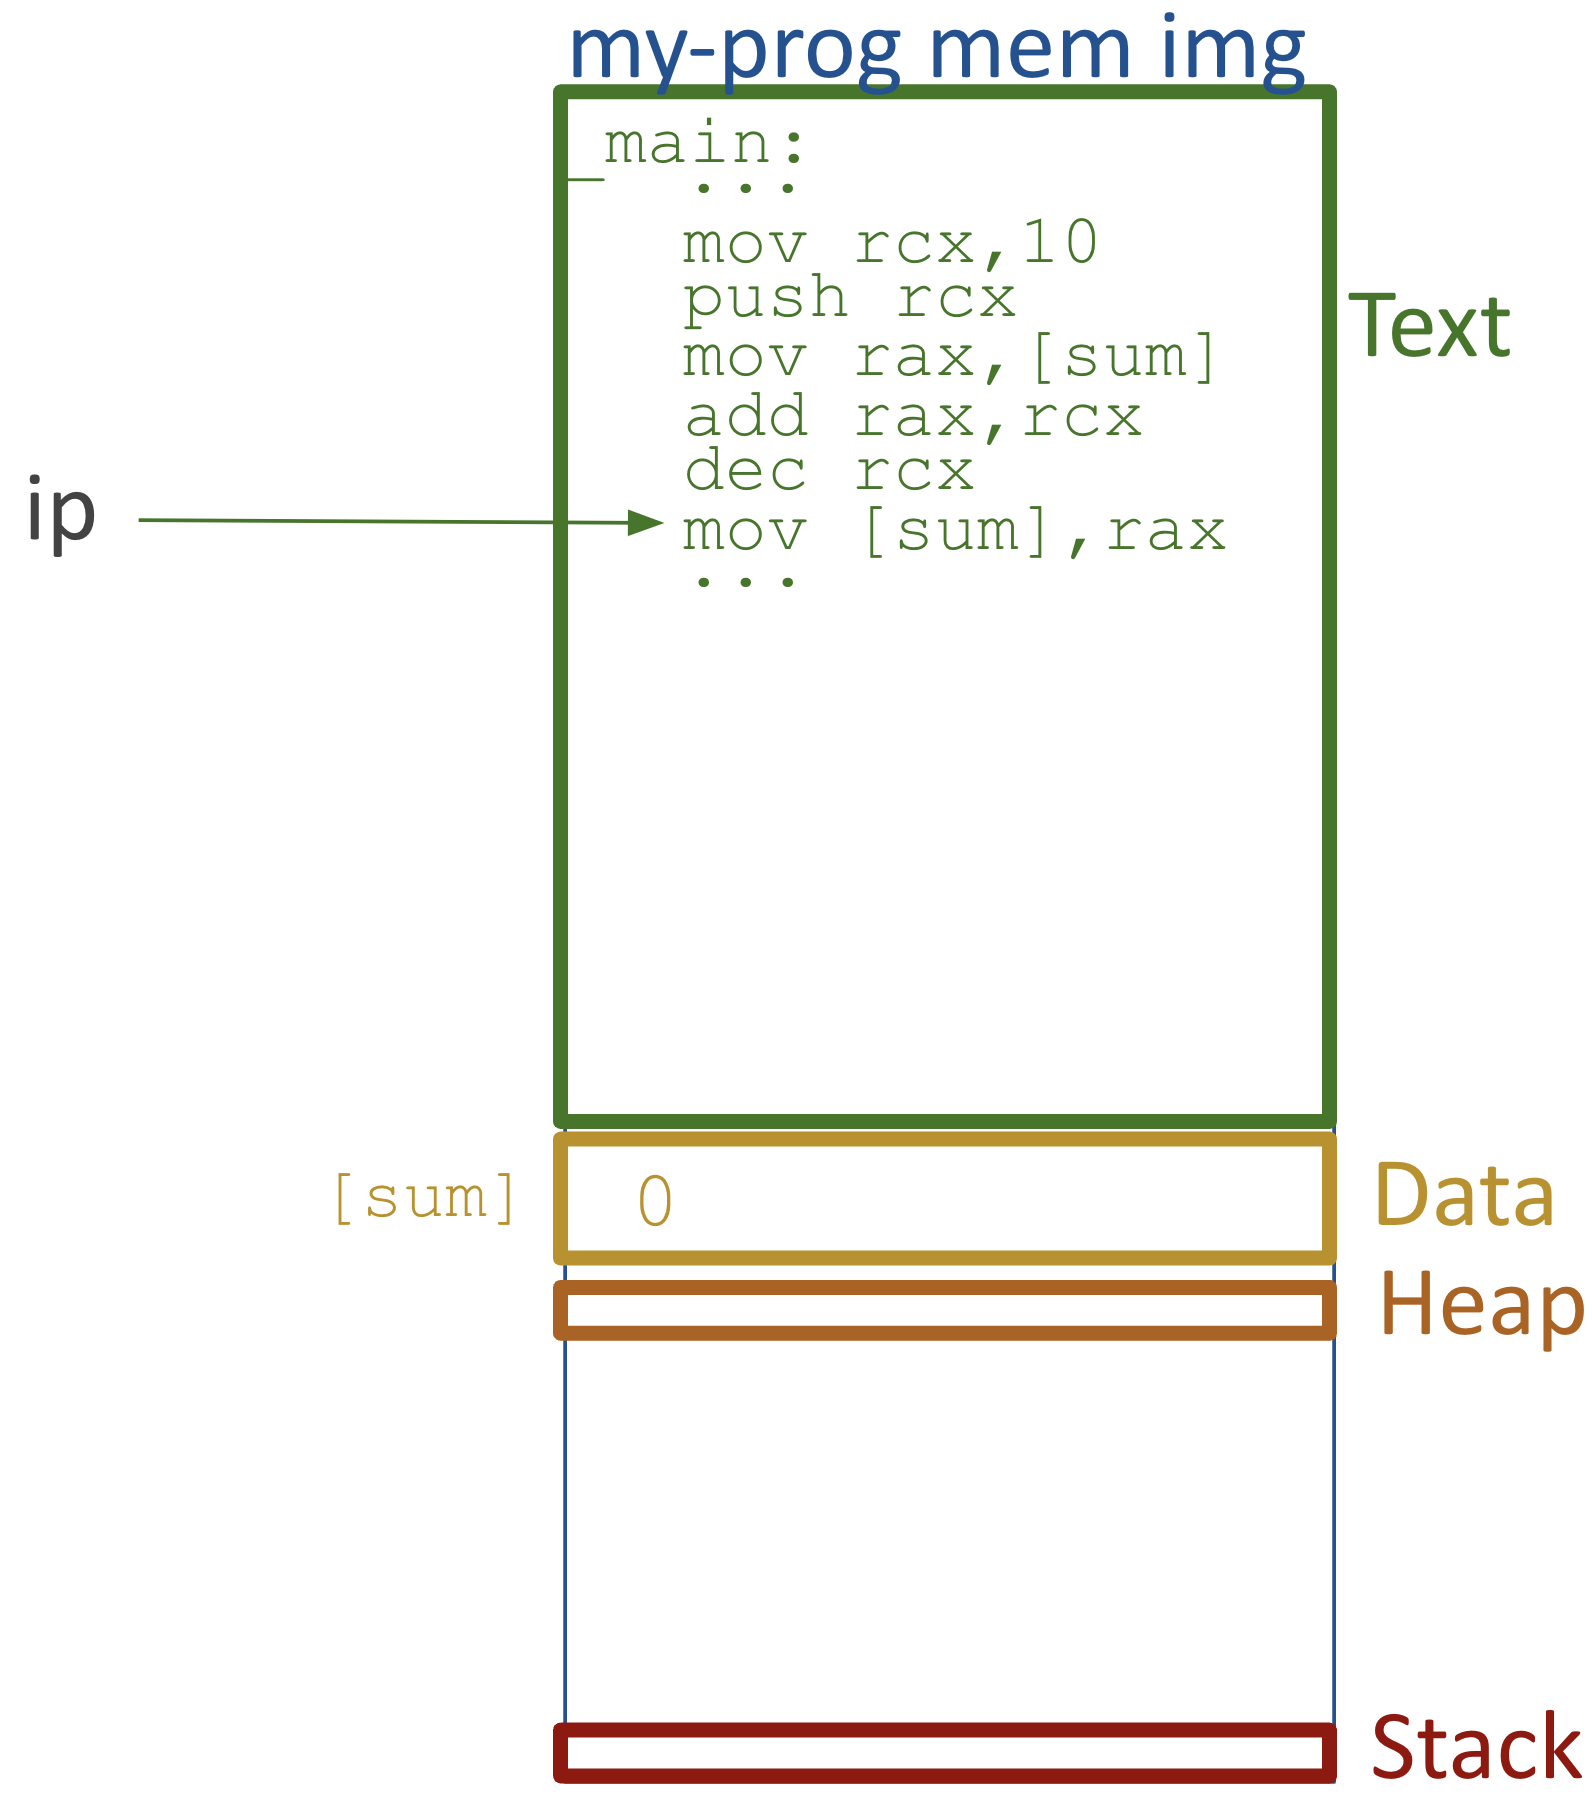
\includegraphics[width=0.75\textwidth]{chapters/L2/images/stack.png}
\end{center}
\end{minipage}

\subsubsection{Stack Frames}
Each function call creates its own \emph{stack frame}, a self-contained section that isolates the function's local data. This segmentation helps maintain the correct scope and lifetime for local variables and ensures that return addresses are preserved. The following diagram illustrates the organization of stack frames during nested function calls:

\begin{center}
    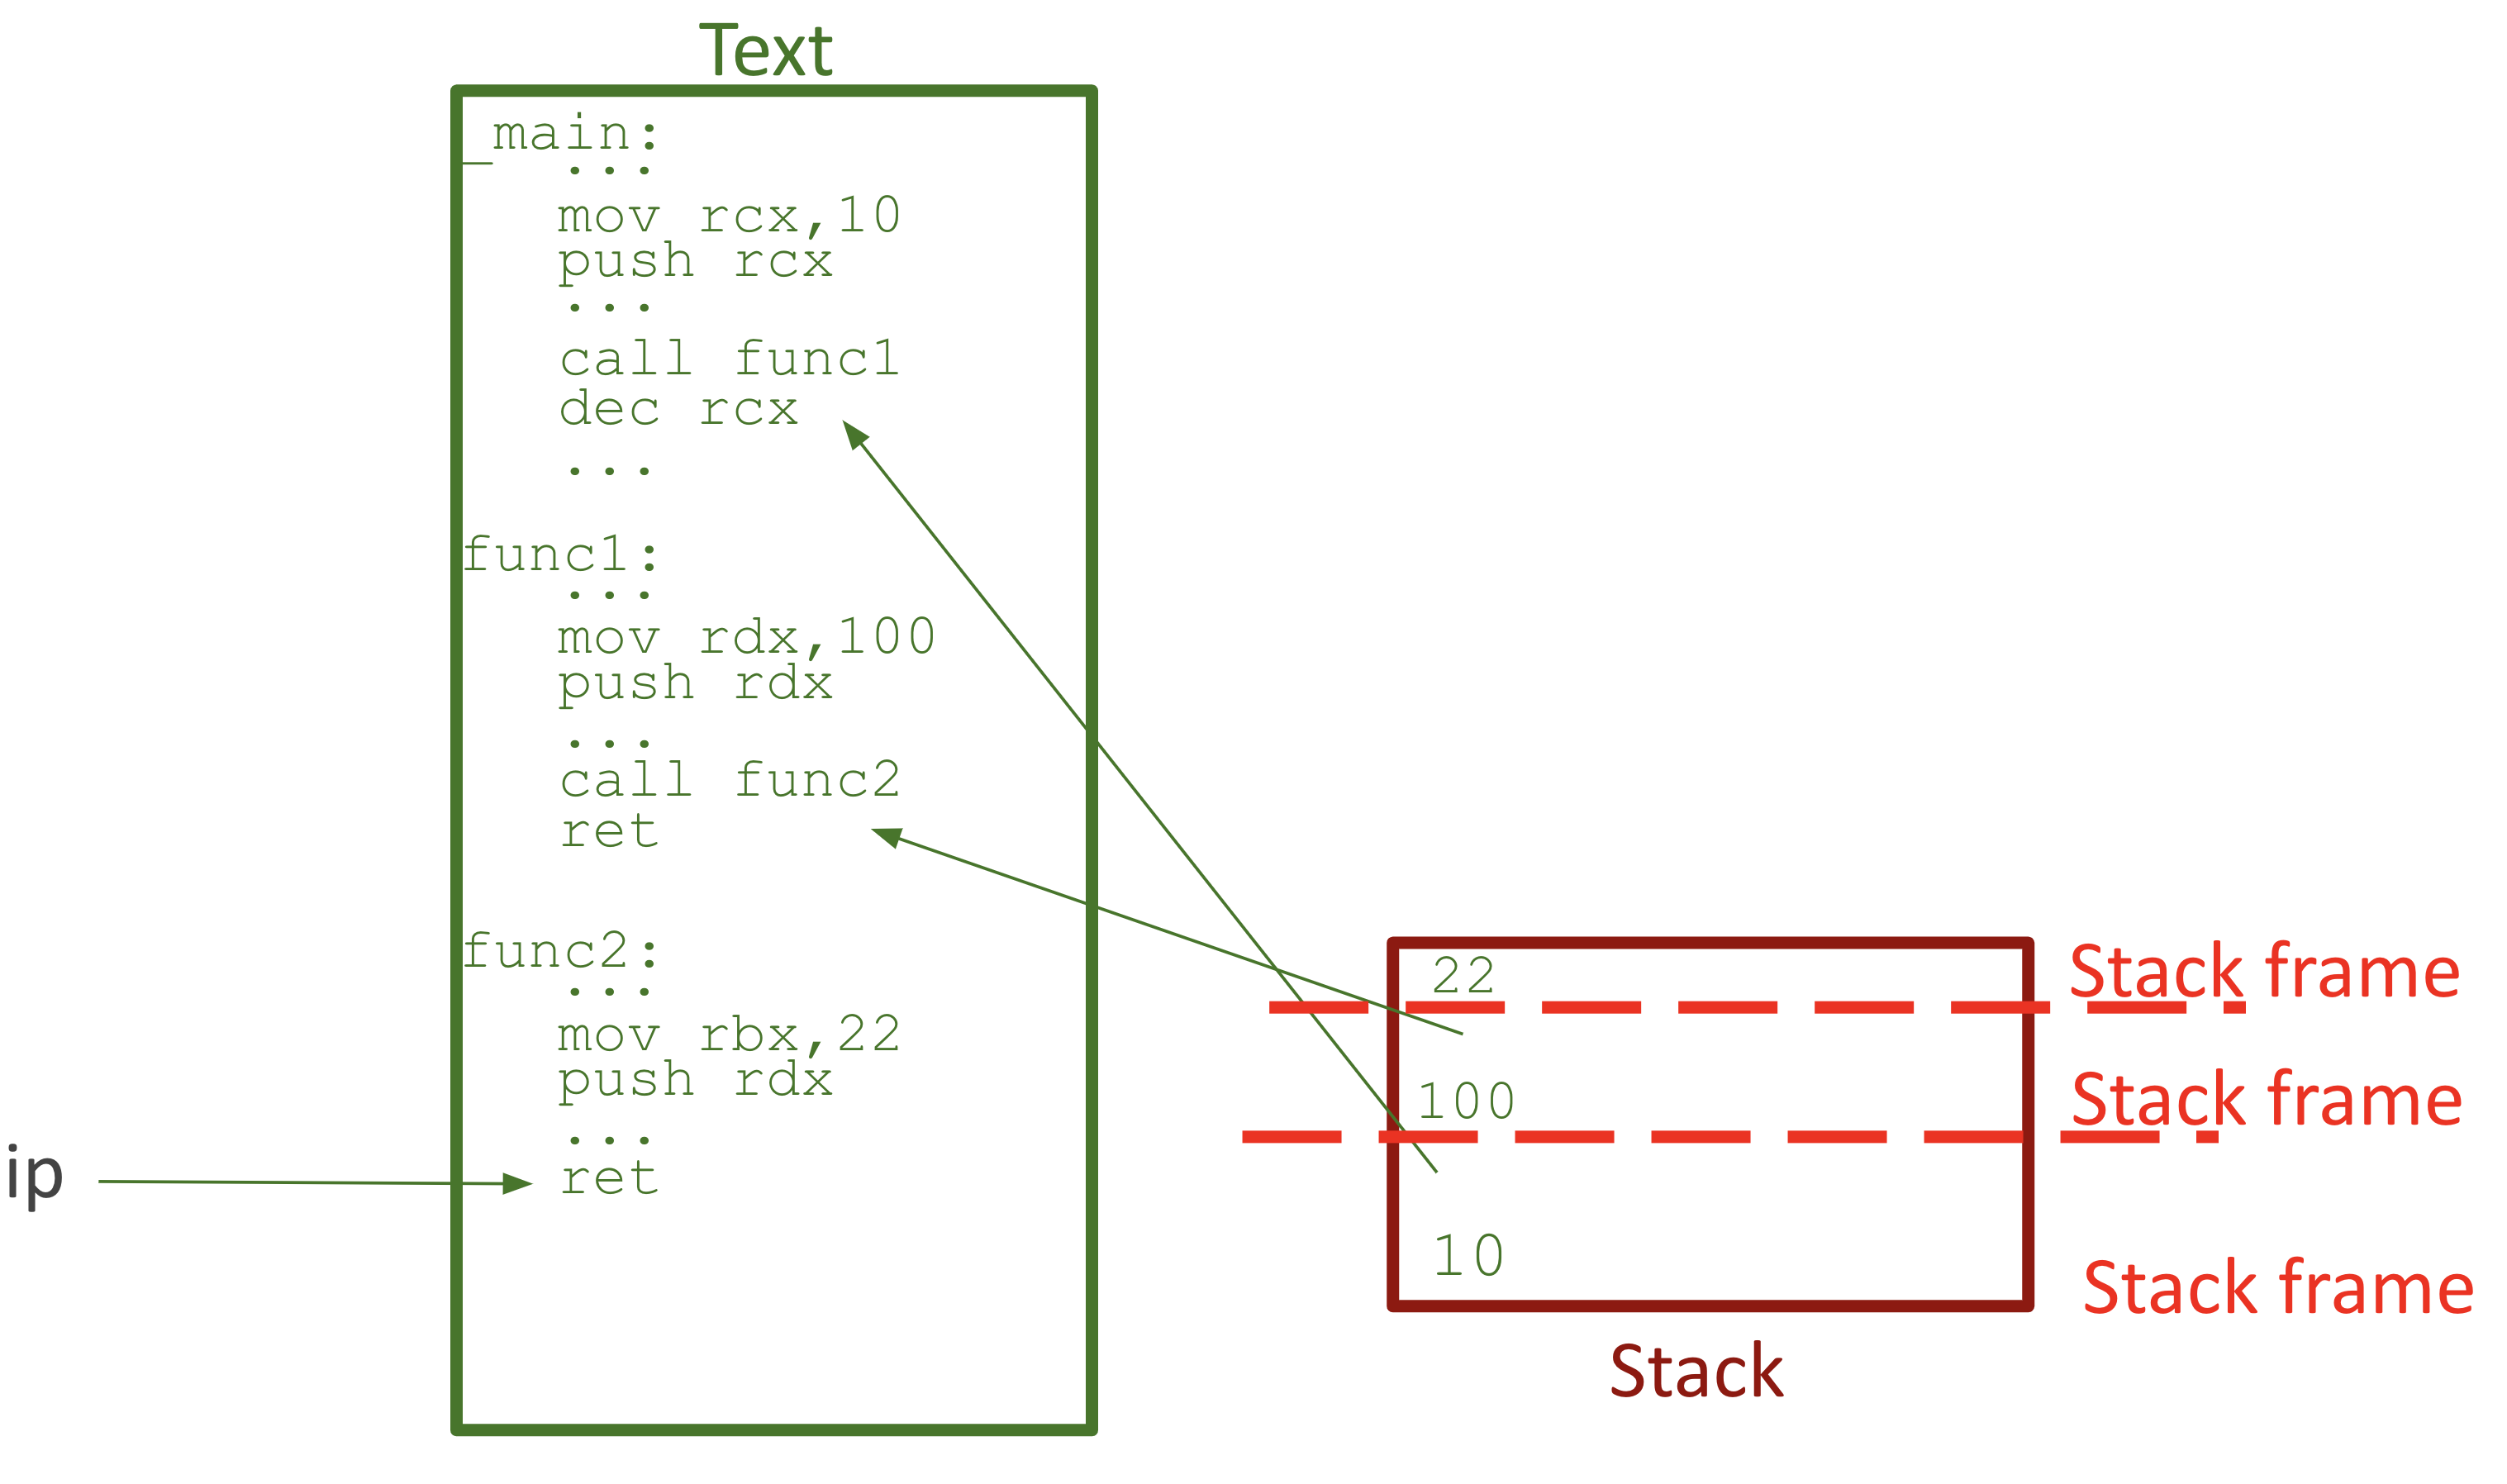
\includegraphics[width=0.65\textwidth]{chapters/L2/images/frames.png}
\end{center}

\subsection{Heap Memory}
The heap is used for dynamic memory allocation, where memory is allocated and deallocated as needed during runtime. Unlike the stack:
\begin{itemize}
  \item[-] \textbf{Manual vs. Automatic Management:} In languages such as C or C++, the programmer is responsible for explicitly allocating (using \texttt{malloc} or \texttt{new}) and deallocating (using \texttt{free} or \texttt{delete}) heap memory. In contrast, some modern languages employ automatic garbage collection.
  \item[-] \textbf{Growth Direction:} The heap typically grows upward, from lower to higher memory addresses.
  \item[-] \textbf{Lifetime:} Data allocated on the heap persists beyond the scope of the function that created it, until it is explicitly freed or garbage collected.
\end{itemize}

\subsection{Data and Text Segments}

\textbf{Text Segment:}  
This segment contains the program's executable code and constant values. Its read-only nature helps prevent inadvertent modifications during execution.
\vspace{0.5em}
\textbf{Data Segment:}  
This segment holds global and static variables. It is divided into:
\begin{itemize}
  \item[-] \textbf{Initialized Data:} Variables that have been assigned an initial value at compile time.
  \item[-] \textbf{Uninitialized Data (BSS):} Variables that are declared but not explicitly initialized; these are automatically set to zero at program startup.
\end{itemize}

\begin{definition}[CPU Registers]
Two registers are critical for process execution:
\begin{itemize}
  \item[-] \textbf{Instruction Pointer (IP):} Points to the next instruction in the text segment.
  \item[-] \textbf{Stack Pointer (SP):} Points to the top of the stack.
\end{itemize}
\end{definition}

\begin{definition}[Process and Thread Identifiers]
\leavevmode\\ % Ensures LaTeX enters vertical mode before inserting a newline
A process is considered to be \emph{running} if at least one of its threads is executing; otherwise, it is not running.
\begin{itemize}
  \item[-] \textbf{Process ID (PID):} A unique identifier assigned to each process.
  \item[-] \textbf{Thread ID (TID):} A unique identifier for each thread, which may be unique within a process or across the entire system, depending on the operating system.
\end{itemize}
\end{definition}

\begin{definition}[Resource Sharing]
Processes and threads share system resources such as CPU and memory. Each thread is given the illusion of having exclusive access to the CPU, and each process appears to have dedicated memory, even though these resources are actually shared.
\end{definition}
\vspace{10px}

\begin{definition}[CPU Sharing]
The CPU is time-shared among multiple threads. This virtualization is achieved through context switching, where the CPU rapidly switches between threads, giving each one the impression of exclusive use of the processor.
\end{definition}

\subsubsection{Example: Two Programs Running on a Single Core}
\begin{example}
Consider two programs running on a single-core processor. Each program is assigned a CPU context, which includes register values such as \texttt{rax}, \texttt{rbx}, the stack pointer (SP), and the instruction pointer (IP). When switching between programs, the CPU saves the current context to memory and loads the context of the next program, allowing the programs to resume correctly.
\end{example}

\begin{center}
    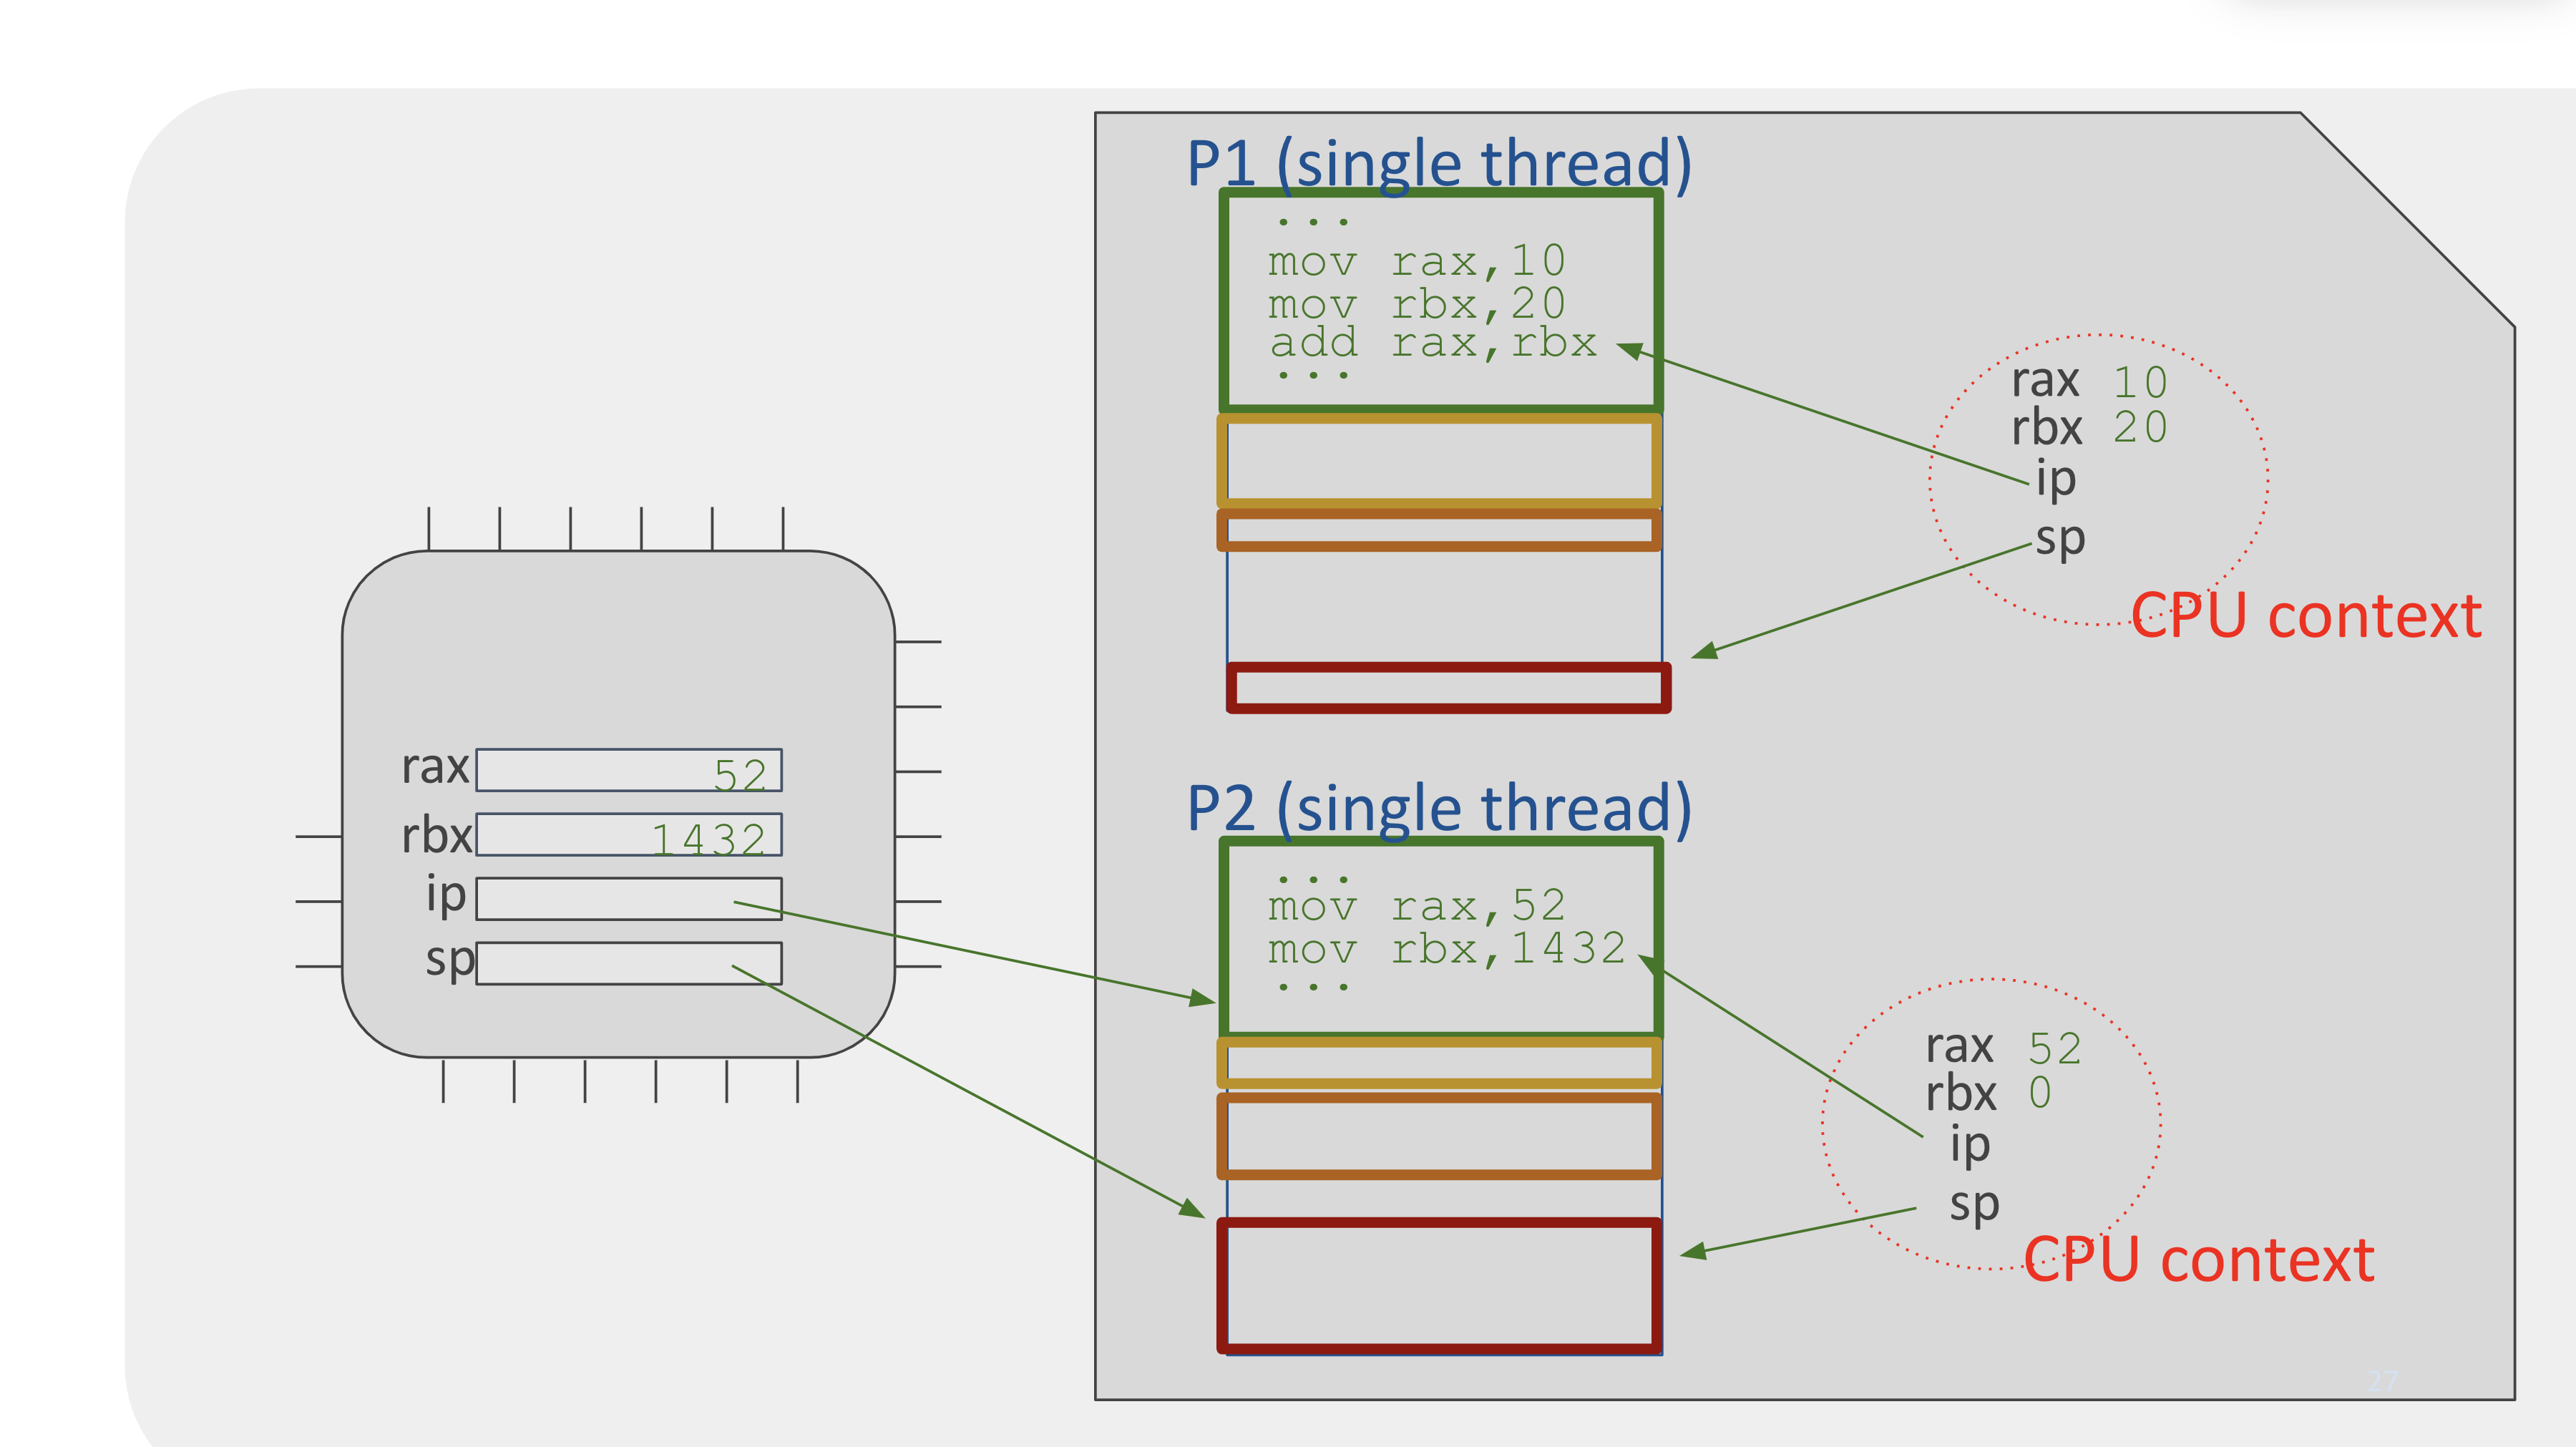
\includegraphics[width=0.8\textwidth]{chapters/L2/images/cpu_context.png}
\end{center}

\begin{definition}[Thread's CPU Context]
A thread's CPU context comprises the values of all CPU registers at the moment it was last executing. In a single-threaded process, this context represents the entire process state.
\end{definition}

\begin{definition}[Context Switching]
Context switching is the process by which the CPU switches from executing one thread to another. It involves:
\begin{enumerate}
    \item Saving the current thread's CPU context to memory.
    \item Restoring the CPU context of the thread to be executed next.
    \item[] Each thread has the illusion that it's occupying the CPU \textbf{alone}.
\end{enumerate}
This mechanism enables CPU virtualization but introduces performance overhead due to additional memory accesses.
\end{definition}
\vspace{10px}
\begin{definition}[Process]
A process is defined by:
\begin{itemize}
    \item A unique Process ID (PID).
    \item A memory image that includes the text, data, heap, and stack segments.
    \item The CPU contexts of each thread within the process.
    \item Associated resources such as file descriptors.
\end{itemize}
\end{definition}
\textit{Remark: If two threads belong to the same process, does each have its own CPU context, or do they share one? The answer is that each thread should be able to continue its execution independently.}
\vspace{10px}
\begin{definition}[Memory Sharing]
Memory in a system is space-shared among processes; however, virtualization ensures that each process operates within its own isolated address space. This is achieved through virtual-to-physical address translation.
\end{definition}
\vspace{10px}
\begin{definition}[Virtual and Physical Addresses]
Virtual addresses allow processes to operate as if they have exclusive access to memory. For example, two processes might both use the virtual address \texttt{0x400000}; however, these addresses map to different physical addresses:
\begin{itemize}
  \item[-] Process \( P_1 \): Virtual \texttt{0x400000} \(\rightarrow\) Physical \texttt{0x1234AFF8}
  \item[-] Process \( P_2 \): Virtual \texttt{0x400000} \(\rightarrow\) Physical \texttt{0xABCD5678}
\end{itemize}
\end{definition}
\vspace{10px}
\begin{definition}[Virtual Address Space]
Each process is allocated its own virtual address space, which is shared among all its threads. This abstraction allows developers to ignore the complexities of physical memory allocation.
\end{definition}
\vspace{10px}
\begin{definition}[Address Translation]
Address translation is the process by which a virtual memory address is converted into a physical memory address. While essential for memory virtualization, this translation incurs a performance cost.
\end{definition}

\subsection{Stack Smashing}
Stack smashing is a type of buffer overflow vulnerability where an attacker deliberately overwrites parts of the memory on the call stack. This typically happens when a program writes more data into a fixed-size buffer than it can accommodate, thereby corrupting adjacent memory areas such as the function's return address.

\paragraph{How It Works:}
When a function is called, a stack frame is created that contains local variables, return addresses, and other control data. If a buffer does not have proper bounds checking, an input exceeding the buffer's capacity can overflow into these critical areas. For example:
\begin{enumerate}
    \item A fixed-size buffer is allocated on the stack.
    \item Excess input data overwrites memory beyond the buffer.
    \item The return address (or other control data) is corrupted.
    \item On function return, control is transferred to an address chosen by the attacker, potentially executing malicious code.
\end{enumerate}
\subsection{Summary: CPU and Memory Virtualization}
\begin{itemize}
    \item \textbf{CPU Virtualization:} Threads time-share the CPU through context switching, which gives each thread the illusion of exclusive CPU access.
    \item \textbf{Memory Virtualization:} Processes space-share memory via virtual-to-physical address translation, ensuring that each process operates in its own isolated address space.
\end{itemize}

\subsection{Conclusion}
Modern operating systems are designed to enable multiple programs to share CPU and memory resources seamlessly. Through context switching and address translation, both the CPU and memory are effectively virtualized. This abstraction simplifies development, as compilers and developers can design programs without needing to manage these low-level resource-sharing details directly.


